\documentclass[a4paper]{article}
\usepackage[left=2cm,right=2cm,top=3cm,bottom=3cm]{geometry}
\usepackage[T1]{fontenc}
\usepackage{amsmath}
\usepackage{mathtools}
\usepackage{amssymb}
\usepackage{indentfirst}
\usepackage{graphicx}
\usepackage{algorithm}
\usepackage{algorithmic}
\usepackage{amsthm}

\graphicspath{ {./images/} }
\newtheorem{theorem}{Theorem}
\let\conjugate\overline


\title{\textbf{Pracownia z Analizy Numerycznej}\\{\Large Sprawozdanie do zadania P1.7}}
\author{Mateusz Leonowicz}

\begin{document}
\maketitle

\section{Wstęp}
    Wiele problemów w matematyce, fizyce czy informatyce sprowadzić można do wyznaczenia miejsc
    zerowych danego równania algebraicznego. Często nie wystarczy nam prosta analiza funkcji, a
    jedyne co możemy zrobić, to obliczenie jej wartości w danej, skończonej liczbie punktów jej dziedziny.
    Dlatego temat ten stał się jednym z fundamentalnych zagadnień analizy numerycznej, dzięki czemu
    powstało wiele metod iteracyjnych, które oczywiście mają swoje zalety i wady.
    
    \vspace{5mm}

    Celem tego sprawozdania jest przedstawienie metod obliczania pierwiastków wielomianów w postaci
    \[ax^3 + bx^2 + cx + d = 0 \qquad a, b, c, d \in \mathbb{R}\]
    które pozwalają komputerom na uzyskanie wyników z kontrolowanym błędem. Przedstawię trzy metody numeryczne oraz 
    rozwiązania z użyciem wzorów Cardano. Opiszę ich działadnie i charakterystykę, a następnie umieszczę ich porównanie
    razem z podsumowaniem.

    Wszystkie testy przeprowadzane będą z użyciem języka do analizy numerycznej Julia.
    
\tableofcontents

\newpage
\section{Metoda Newtona}
    Niech $f(x)$ będzie funkcją, której miejsce zerowe chcemy wyznaczyć. Niech $\alpha$ będzie takim zerem, a $x$
    jego przybliżeniem. Z twierdzenia Taylora, wiemy, że przybliżenie funkcji $f$, możemy zapisać w postaci:
    \[
        0 = f(\alpha) = f(x + e) = f(x) + ef'(x) + \frac{f''(\xi)}{2!}e^2 \qquad \xi \in \text{interv}(x, \alpha) 
    \tag{1}\]

    Jeśli nasz wyraz $\frac{f''(\xi)}{2!}e^2$ będzie dostatecznie mały, to możemy go pominąć i rozwiązać równanie 
    względem $e$, co daje nam:
    \[
        e = \frac{-f(x)}{f'(x)}  
    \]

    Jeśli $x$ jest dostatecznie dobrym przybliżeniem $\alpha$, to $x - e$ będzie jeszcze lepszym przybliżeniem tego
    pierwiastka. Na tej różnicy opiera się metoda Newtona, która po wybraniu startowego przybliżenia $x_0$ zera $\alpha$
    polega na stosowaniu rekurencyjnego wzoru:
    \[
        x_{n+1} = x_n - \frac{f(x)}{f'(x)} \qquad n \geq 0
    \tag{2}\]

    Dobranie startowego punktu $x_0$ w tej metodzie jest bardzo istotne, gdyż metoda Newtona nie zawsze jest zbieżna.
    Jeśli dobierzemy odpowiednio punkt początkowy będziemy mieli zbieżność kwadratową, z wyjątkiem przypadków, gdy 
    istnieją wielokrotne zera funkcji. Wtedy otrzymamy zbieżność liniową.

    \vspace{5mm}

    Metoda Newtona opiera się na linearyzacji funkcji $f$, co pozwala nam na dobre przybliżanie wartości funkcji w małym
    otoczeniu punktu $x$. Możemy więc rozumieć tę metodę, jako przybliżanie miejsc zerowych funkcji za pomocą jej stycznych,
    co oczywiście niesie za sobą groźbę rozbieżności.

    \vspace{10mm}

    \begin{figure}[h]
        \centering
        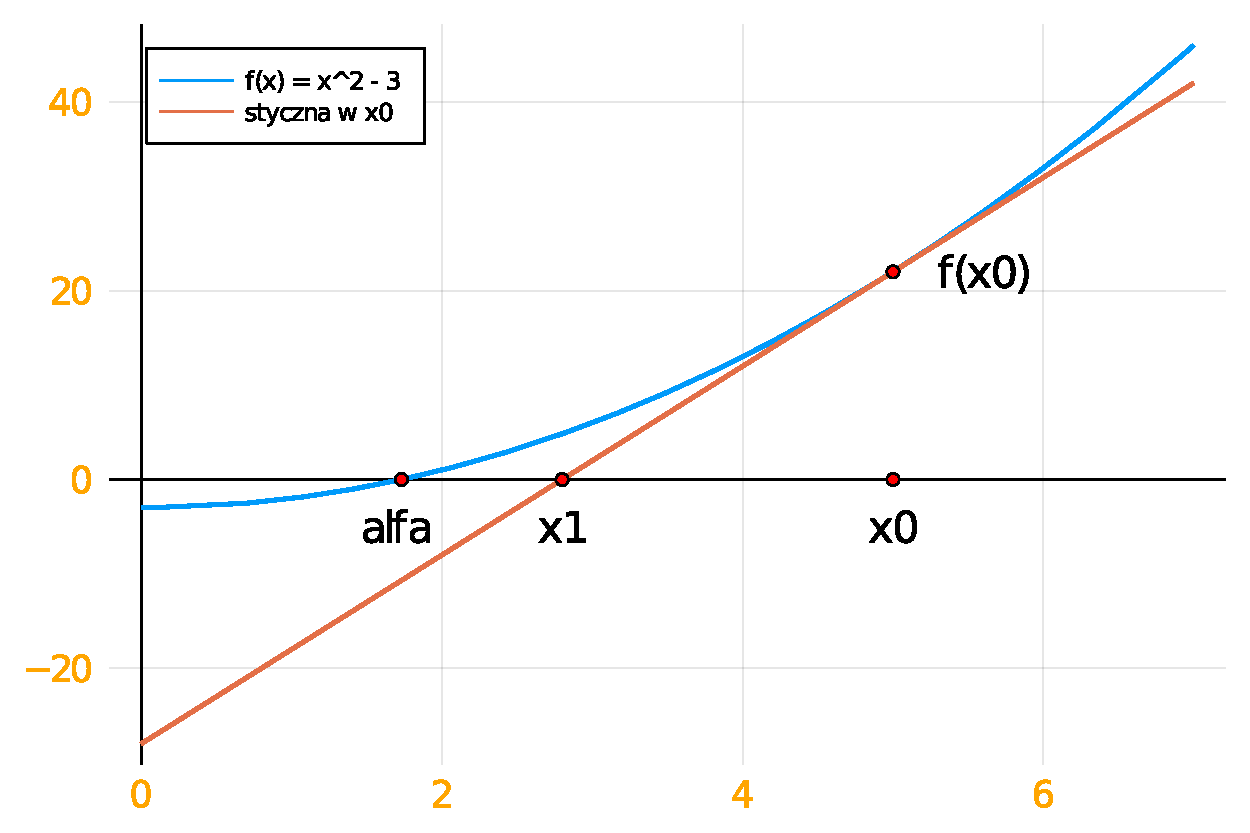
\includegraphics[width=12cm]{newtonPlot}
        \caption{Interpretacja geometryczna metody Netwona}
    \end{figure}

\newpage
\section{Metoda bisekcji}
    Niech $f$ będzie funkcją ciągłą w przedziale $[a,b]$ i jeśli $f(a)f(b) < 0$, czyli funkcja zmienia znak na końcach przedziałów, to
    ta funkcja musi mieć zero w przedziale $(a,b)$ i jest to oczywiście konsekwencja twierdzenia Darboux. Możemy więc zmniejszyć nasz
    przedział o połowę wybierając punkt $c$, taki że $f(c)f(a) < 0$ lub $f(c)f(b) < 0$. Uzyskaliśmy nowy przedział, w którym wiemy, że
    znajduje się nasze miejsce zerowe. Na tym rozumowaniu opiera się metoda biskecji, którą wyrazić można następującym algorytmem:

    \begin{algorithm}
    \caption{Szukanie pierwiastka funkcji $f$}
    \begin{algorithmic}
    \REQUIRE $\epsilon\ a_0\ b_0\ M \quad \text{takie, że} \quad f(a_0)f(b_0) < 0$
        \STATE $n \leftarrow 1$
        \STATE $left \leftarrow a_0$
        \STATE $right \leftarrow b_0$
        \WHILE{$n < M$}
        \STATE $c = \frac{left + right}{2}$
        \IF{$f(c) = 0 \vee \lvert left - right \lvert < \epsilon$}
        \STATE $\text{pierwiastkiem jest}\ c$
        \ELSE
        \STATE $n \leftarrow n + 1$
        \ENDIF
        \IF{$f(left)f(c) < 0$}
        \STATE $left \leftarrow c$
        \ELSE
        \STATE $right \leftarrow c$
        \ENDIF
        \ENDWHILE
        \end{algorithmic}
    \end{algorithm}

    Algorytm uwzględnia trzy kryteria zakończenia obliczeń, ponieważ inaczej istniałoby
    ryzyko zapętlenia. Pierwszym jest oczywiście znalezienie takiego punkt $c$, że $f(c) = 0$. Drugim z nich jest 
    skończona liczba iteracji wyrażona zmienną $M$. Oprócz tego, obliczenia są przerywane, 
    jeżeli błąd jest dostatecznie mały, tj. mniejszy od $\epsilon$. Łatwo znaleźć przykłady funkcji w których
    brak któregoś z kryterów mógłby prowadzić do bardzo błędnych wyników.

    \begin{figure}[h]
        \centering
        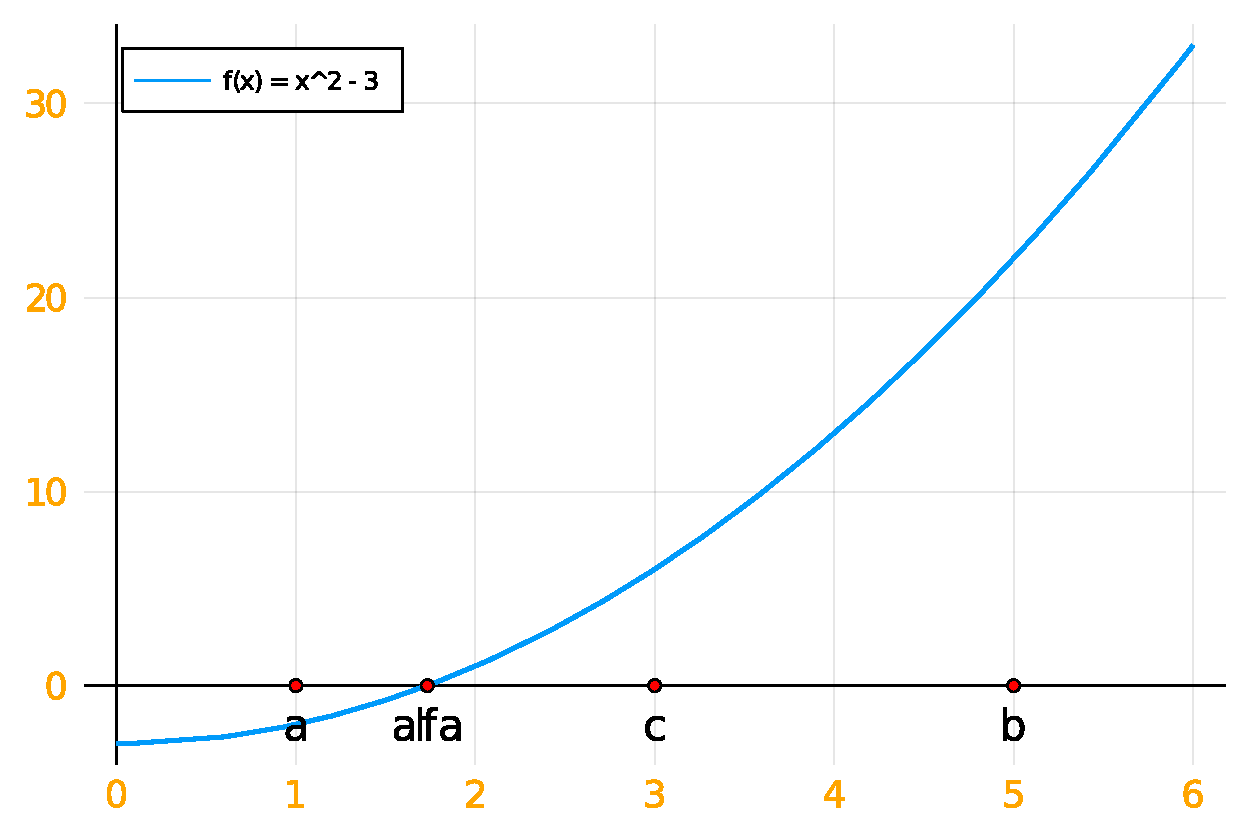
\includegraphics[width=12cm]{bisectionPlot}
        \caption{Interpretacja geometryczna metody bisekcji}
    \end{figure}

\newpage
\section{Metoda Bairstowa}
    Wymienione metody do tej pory, oprócz oczywistych problemów z wybraniem początkowych wyrazów, czy niejednolitą zbieżnością, mają
    jedną o wiele poważniejszą dla nas wadę. W ich akutalnej postaci, jeśli nasza funkcja $f$ będzie miała pierwiastki zespolone, to
    ich nie wyznaczymy. Do tego potrzebujemy bardziej zaawansowanego i ogólnego algorytmu. Najpierw przedstawię 
    kilka letmatów, które przydadzą się do wyprowadzenia metody Bairstowa.
    \begin{theorem}
        Wielomian stopnia n ma dokładnie n pierwiastków w przestrzeni zespolonej, gdy każdy z nich liczony jest tyle razy, ile wynosi jego krotność.
    \end{theorem}
    
    \begin{theorem}
        Jeśli wielomian $w(x)$ stopnia $n \in \mathbb{N}$ ma współczynniki 
        $a_i \in \mathbb{R},\ 0 \leq i \leq n$, oraz $\alpha \in \mathbb{C} \setminus \mathbb{R}$ jest jego 
        miejscem zerowym, to $\conjugate{\alpha}$ też jest jego miejscem zerowym, a iloczyn
        kwadratowy $(x - \alpha)(x - \conjugate{\alpha})$ dzieli bez reszty wielomian $w(x)$.
    \end{theorem}
    \begin{proof}
        Mamy wielomian $w(x) = a_{n}x^n + a_{n-1}x^{n-1} + \ldots + a_{0}x^0$, oraz z założenia wiemy, że
        $w(\alpha) = 0$. Korzystając z dwóch własności sprzężenia $\conjugate{x + y} = \conjugate{x} + \conjugate{y}$,
        ${\conjugate{xy} = \conjugate{x}\conjugate{y}}$ otrzymujemy wprost równość: $w(\conjugate{\alpha})$. Ponieważ
        $\alpha$ jest pierwiastkiem nierzeczywistym, to $\alpha \neq \conjugate{\alpha}$. Z twierdzenia o reszcie, wynika, że
        iloczyn $(x - \alpha)(x - \conjugate{\alpha})$ dzieli nasz wielomian bez reszty.
    \end{proof}

    \begin{theorem}
        Dzielenie wielomianu 
        \[
            w(x) = a_{n}x^n + a_{n-1}x^{n-1} + \ldots + a_{0}x^0
        \]
        Przez wielomian w postaci $(x^2 - ux - v) \ \ u,v \in \mathbb{C}$ daje iloraz i resztę równe:
        \[
            \begin{array}{c}
                \phi(x) = b_{n}x^{n-2} + b_{n-1}x^{n-3} + \ldots + b_{2}x^0 \\
                r(x) = b_{1}(z - u) + b_{0}
            \end{array}
        \]
        Których współczynniki dane są rekurencyjnym wzorem:
        \[
            b_{n+1} = b_{n+2} = 0, \qquad b_k = a_k + ub_{k+1} + vb_{k+2} \qquad (n \leq k \leq 0).  
        \tag{3}\]
        Dowód jest dość prosty i polega na porównaniu współczynników po obu stronach równania:
        \[
            w(x) = \phi(x)(x^2 - ux - v) + r(x)  
        \]
    \end{theorem}

    Dla każdego wielomianu $w$ stopnia $n \leq 2$ znajdziemy więc takie $u$ i $v$, że nasz wielomian $(x^2 - ux -v)$ będzie dzielił
    $w$ bez reszty. Na szukaniu tych rzeczywistych czynników opiera się metoda Bairstowa. W $r(x)$ nasze współczynniki $b_0$ i $b_1$
    zależą od $u$ i $v$, więc zapiszmy:
    \[
        b_0(u, v) = 0 \qquad b_1(u, v) = 0  
    \]
    Są to równania nieliniowe, dwuargumentowe. Szukamy więc takich poprawek oznaczonych $\delta u$ i $\delta v$, które spełniałyby równanie:
    \[
        b_0(u + \delta u, v + \delta v) = b_1(u + \delta u, v + \delta v) = 0  
    \]
    Z twierdzenia Taylora możemy zlinearyzować powyższe równości, co daje:
    \[
        \begin{array}{c}
            b_0(u, v) + \frac{\partial b_0}{\partial u}\delta u + \frac{\partial b_0}{\partial v}\delta v = 0  \\\\
            b_1(u, v) + \frac{\partial b_1}{\partial u}\delta u + \frac{\partial b_1}{\partial v}\delta v = 0  
        \end{array}
    \tag{4}\]
    Zdefiniujmy więc wyrazy pomocnicze, które oczywiście spełniają rekurencyjną zależność z (3):
    \[
        c_k = \frac{\partial b_k}{\partial u} \qquad (0 \leq k \leq n) 
    \]
    Podstawiając do równań z (4) i uzależniając równania od $\delta v$ i $\delta u$ otrzymujemy:
    \[
        \begin{array}{c}
            \delta u = (c_1b_1 - c_2b_0)\frac{1}{J} \\\\
            \delta v = (c_1b_0 - c_0b_1)\frac{1}{J} \\\\
            J = c_0c_2 - c_1^2
        \end{array}
    \]
    Otrzymaliśmy więc wzór na lepsze przybliżenie naszej pary $(u, v)$.

\newpage
\section{Wzory Cardano}
    Do rozwiązywania takich problemów w przypadku wielomianów 3 stopnia posłużyć również mogą wzory dające nam wprost
    pierwiastki funkcji. Wzory Cardano są dość skomplikowane matematycznie, ale są proste do wyprowadzenia i udowodnienia,
    dlatego przedstawię krótki opis. Niech $f$ będzie wielomianem 3 stopnia:
    \[
        f(x) = ax^3 + bx^2 + cx + d
    \]
    wtedy możemy przekształcić naszą funkcję $f$ do alternatywnej postaci
    \[
        \begin{array}{c}
            g(y) = y^3 + Qy - 2R \\ \\
            y = x + \frac{b}{3a }, \ Q = \frac{3ac - b^2}{9a^2}, \ R = \frac{9abc - 27a^2d - 2b^3}{54a^3} 
        \end{array}
    \]
    Teraz, niech $y = (u + v)$, gdzie $uv = -Q$. Przekształcając otrzymujemy nową postać naszej funkcji.
    \[
        g(u + v) = u^6 - 2Ru^3 - Q^3
    \]
    Widzimy, że otrzymujemy funkcję kwadratową względem $u^3$, więc dostajemy równości:
    \[
        u^3 = \frac{2R \pm \sqrt{4Q^3 + 4R^2}}{2} = R \pm \sqrt{Q^3 + R^2}
    \]
    Niech $u^3 = R + \sqrt{Q^3 + R^2}$. Mamy wtedy:
    \[
        v^3 = -\frac{Q^3}{u^3} = R - \sqrt{Q^3 + R^2}
    \]
    Jeśli weźmiemy $u^3 = R - \sqrt{Q^3 + R^2}$, to analogicznie otrzymamy $v^3 = R + \sqrt{Q^3 + R^2}$. 
    Bez straty ogólności przyjmijmy, że
    \[
        \begin{array}{c}
            S = \sqrt[3]{u^3} = \sqrt[3]{R + \sqrt{Q^3 + R^2}} \\
            T = \sqrt[3]{v^3} = \sqrt[3]{R - \sqrt{Q^3 + R^2}}
        \end{array}
    \]
    Wtedy istnieje oczywiście 9 kombinacji dla wartości $v, u$, ale tylko 3 z nich pasują do naszych
    warunków. Są to 
    \[
        \begin{array}{c}
            u = S \land v = T \\
            u = (-\frac{1}{2} + \frac{i\sqrt{3}}{2})S \land v = (-\frac{1}{2} - \frac{i\sqrt{3}}{2})T \\
            u = (-\frac{1}{2} - \frac{i\sqrt{3}}{2})S \land v = (-\frac{1}{2} + \frac{i\sqrt{3}}{2})T
        \end{array}
    \]
    Nasze pierwiastki zespolone $x_0, x_1, x_2$ równe więc są:
    \[
        \begin{array}{c}
            x_0 = S + T - \frac{b}{3a} \\
            x_1 = -\frac{S + T}{2} - \frac{b}{3a} + \frac{i\sqrt{3}}{2}(S - T) \\
            x_2 = -\frac{S + T}{2} - \frac{b}{3a} - \frac{i\sqrt{3}}{2}(S - T)
        \end{array}
    \]

    Wzory te dają nam pierwiastki wielomianu najszybciej Może okazać się jednak, że proste operacje arytmetyczne,
    które wykonywane są po drodze bardzo wpłyną na nasz wynik dając przekłamane zera. Głównie problemem okazać się 
    może utrata cyfr znaczących przy odejmowaniu dwóch bliskich sobie liczb.

\newpage
\section{Testy numeryczne}
    Tę sekcję poświęcę na porównanie opisanych przeze mnie metod poprzez zestawienie ze sobą wyników zbieżnością
    do pierwiastków wybranych przeze mnie wielomianów 3-go stopnia. Metodę biskecji potraktuję raczej jako ciekawostkę
    i umieszczę ją tylko w pierwszych testach, ponieważ sam problem doboru przedziału dyskwalifikuje ją jako 
    efektywną metodę. Dodatkowo, po zakończeniu algorytmów metod biskecji i Newtona z uzyskanego pierwiastka
    obliczam dwa pozostałe dzieląc mój początkowy wielomian przez otrzymane przybliżenie.

    Najpierw przedstwię wynki wszystkich stworzonych przeze mnie różnorodnych testów, które dają dość obiektywny 
    pogląd na efektywność algorytmów. W testach znajdować się będą tabelki dla każdej metody, w których umieszczę przybliżenie
    mojego głównego pierwiastka i wartość funkcji w tym punkcie. Dodatkowo dla interesujących iteracji dodam ilość cyfr znaczących
    każdego przybliżenia.

    Następnie wszystko podsumuję w sekcji umieszczonej po testach, w której wyciągnę wnioski z uzyskanych wyników. 
    Tam również znajdzie się odpowiedź do naszego zadania, oraz jej uzasadnienie.

    \vspace{5mm}

    Wszystkie obliczenia oraz dodatkowe wykresy umieściłem w jupyterze, w którym zaimplementowana jest całość kodu
    wraz z opisami. Do obliczeń używam 128-bitowej precyzji oraz wyłącznie poprawnie numerycznych algorytmów.

    \vspace{5mm}
        
    Przez C. z. oznaczam liczbe cyfr znaczących, a $e(x)$ oznacza błąd bezwzględny przybliżenia pierwiastka.

    \subsection{Dobór przybliżenia pierwszego pierwiastka}
    Dla metody Newtona będę stosował algorytm do wybierania pierwszego przybliżenia pierwiastka. Polega 
    on na rozpoznaniu, czy pierwiastek rzeczywisty funkcji leży między zerami jej pochodnej, czy poza nimi. Niech
    $f$ będzie wielomianem 3-go stopnia i niech $f'$ będzie jego pochodną. Jeśli $f'$ ma pierwiastki rzeczywiste,
    to niech będą to $x_1 \leq x_2$. Sprawdźmy więc, czy funkcja zmienia znak poza zerami pochodnej. Jeżeli
    \[
        sgn(x_1 - \frac{1}{2}) = sgn(a)  
    \]
    to nasze pierwsze przybliżenie będzie równe $x_1 - \frac{1}{2}$. Jeśli ten warunek nie zachodzi, to 
    sprawdzamy analogicznie dla punktu $x_2 + \frac{1}{2}$. Jeśli funkcja nie zmienia znaku poza tymi punktami, 
    to wybieramy dowolnie punkt między zerami pochodnej. Jeśli nasza pochodna nie ma pierwiastków rzeczywistych, 
    to pozostaje nam dobrać punkt startowy arbitralnie.

\newpage
\subsection{Test 1}
    Prosta funkcja przykładowa, aby zaprezentować sposób prezentacji danych oraz kryteria porównawcze.
    \begin{figure}[h]
        \centering
        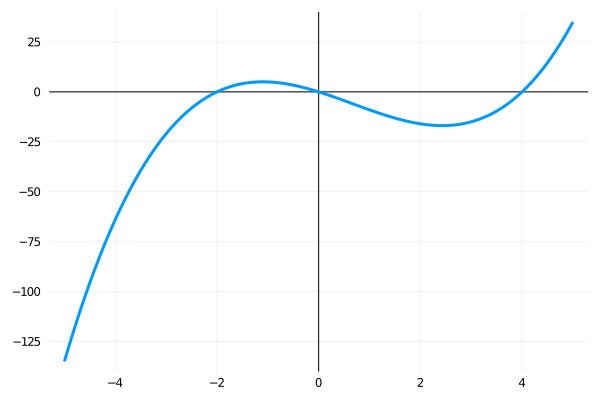
\includegraphics[width=10cm]{1}
        \caption{$f(x) = x^3 - 2x^2 - 8x$}
    \end{figure}
    
    \begin{center}
        Metoda Newtona
    \end{center}
    \begin{center}
        \begin{tabular}{|c|c|c|c|c|c|} 
            \hline
            Iteracja & $x_0$ & $f(x_0)$ & C.z. $x_0$ & C.z. $x_1$ & C.z. $x_2$ \\
            \hline
            1 & 87.40256216597504 & 683055.1593426905 & 0 & 0 & 0 \\
            \hline
            5 & 4 & 0 & inf+ & inf+ & inf+ \\
            \hline
            10 & 4 & 0 & inf+ & inf+ & inf+ \\
            \hline
        \end{tabular}
    \end{center}
        
    \vspace{5mm}

    \begin{center}
        Metoda Bisekcji
    \end{center}
    \begin{center}
        \begin{tabular}{|c|c|c|c|c|c|} 
            \hline
            Iteracja & $x_0$ & $f(x_0)$ & C.z. $x_0$ & C.z. $x_1$ & C.z. $x_2$ \\
            \hline
            1 & 2.500000 & -8.125000 & 0 & 0 & 0 \\
            \hline
            5 & 4.531250 & 15.722198 & 1 & 0 & 0 \\
            \hline
            10 & 4.018555 & 0.448762 & 2 & 2 & 2 \\
            \hline
            15 & 3.999481 & -0.012448 & 3 & 3 & 3 \\
            \hline
            20 & 3.999982 & -0.000435 & 5 & 5 & 5 \\
            \hline
        \end{tabular}
    \end{center}
    
    \vspace{5mm}

    \begin{center}
        Metoda Bairstowa
    \end{center}
    \begin{center}
        \begin{tabular}{|c|c|c|c|c|c|} 
            \hline
            Iteracja & $x_0$ & $f(x_0)$ & C.z. $x_0$ & C.z. $x_1$ & C.z. $x_2$ \\
            \hline
            1 & -3.14625657737552 & -25.77238332178403 & 0 & 0 & 0 \\ 
            \hline
            5 & -1.5183794715 - 2.1659587805i & 34.78812403 - 0.6466883761i & 0 & 2 & 0 \\ 
            \hline
            10 & -2.0 & 0.0 & inf+ & inf+ & inf+ \\
            \hline
            15 & -2.0 & 0.0 & inf+ & inf+ & inf+ \\
            \hline
        \end{tabular}
    \end{center}

    \vspace{5mm}

    \begin{center}
        Błędy bezwzględne dla wzorów Cardano:
        \[
            e(x_0) = 0 \qquad e(x_1) = 0 \qquad e(x_2) = 0  
        \]
    \end{center}

\newpage
\subsection{Test 2}
    Funkcja, która ma miejsca zerowe odległe od 0, oraz podwójny pierwiastek rzeczywisty.
    \begin{figure}[h]
        \centering
        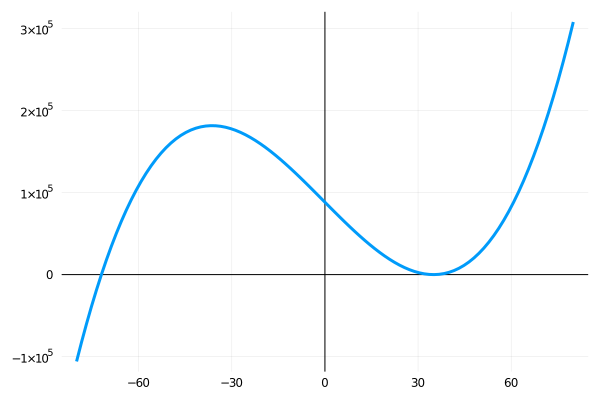
\includegraphics[width=10cm]{2}
        \caption{$f(x) = x^3 + 2x^2 + 3815x - 88200$}
    \end{figure}

    \begin{center}
        Metoda Newtona
    \end{center}
    \begin{center}
        \begin{tabular}{|c|c|c|c|c|c|} 
            \hline
            Iteracja & $x_0$ & $f(x_0)$ & C.z. $x_0$ & C.z. $x_1$ & C.z. $x_2$ \\
            \hline
            1 & 23.11296895543223 & 13439.605853832152 & 0 & 0 & 0 \\
            \hline
            5 & 34.33910684864469 & 46.44676930300225 & 1 & 0 & 0 \\
            \hline
            10 & 34.97947097899548 & 0.04508550349326828 & 2 & 0 & 0 \\
            \hline
            25 & 34.999999399616065 & 3.9879819941898415e-11 & 8 & inf+ & 8 \\
            \hline
            40 & 34.99999999967189 & -1.9895119090292067e-12 & 9 & inf+ & 9 \\
            \hline
        \end{tabular}
    \end{center}
        
    \vspace{5mm}

    \begin{center}
        Metoda Bisekcji
    \end{center}
    \begin{center}
        \begin{tabular}{|c|c|c|c|c|c|} 
            \hline
            Iteracja & $x_0$ & $f(x_0)$ & C.z. $x_0$ & C.z. $x_1$ & C.z. $x_2$ \\
            \hline
            1 & -100 & -510300 & 0 & 0 & 0 \\
            \hline
            5 & -75 & -36300 & 0 & 0 & 0 \\
            \hline
            15 & -72.003173828125 & -36.339313896678505 & 2 & 1 & 1 \\
            \hline
            25 & -72.00000286102295 & -0.032755853497292285 & 6 & 2 & 2 \\
            \hline
        \end{tabular}
    \end{center}
    
    \vspace{5mm}

    \begin{center}
        Metoda Bairstowa
    \end{center}
    \begin{center}
        \begin{tabular}{|c|c|c|c|c|c|} 
            \hline
            Iteracja & $x_0$ & $f(x_0)$ & C.z. $x_0$ & C.z. $x_1$ & C.z. $x_2$ \\
            \hline
            1 & 75.91167528178869 & 247569.41096827542 & 0 & 0 & 0 \\ 
            \hline
            5 & -71.99999999198174 & 9.18010833055059e-5 & 7 & 2 & 2 \\ 
            \hline
            10 & -71.99999999999976 & 2.7679476488628924e-9 & 13 & 3 & 3 \\
            \hline
            20 & -72.0 & 0.0 & inf+ & 6 & 6 \\
            \hline
        \end{tabular}
    \end{center}

    \vspace{5mm}

    \begin{center}
        Błędy bezwzględne dla wzorów Cardano:
        \[
            e(x_0) = 0 \qquad e(x_1) = 0 \qquad e(x_2) = 0  
        \]
    \end{center}

\newpage
\subsection{Test 3}
    Funkcja mająca 2 pierwiastki zespolone i jeden rzeczywisty znacznie oddalony od 0.
    \begin{figure}[h]
        \centering
        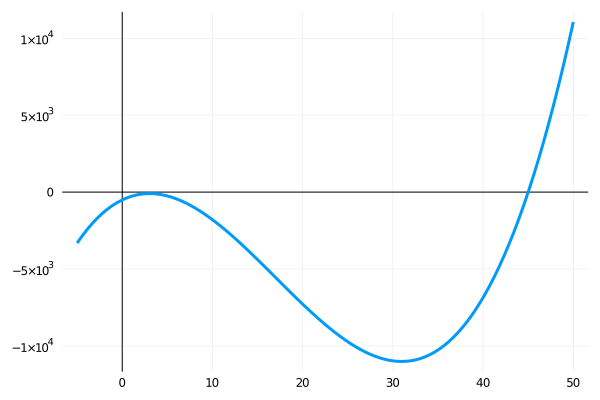
\includegraphics[width=10cm]{3}
        \caption{$f(x) = x^3 - 51x^2 + 281.25x - 506.25$}
    \end{figure}

    \begin{center}
        Metoda Newtona
    \end{center}
    \begin{center}
        \begin{tabular}{|c|c|c|c|c|c|} 
            \hline
            Iteracja & $x_0$ & $f(x_0)$ & C.z. $x_0$ & C.z. $x_1$ & C.z. $x_2$ \\
            \hline
            1 & 289.1961123377604 & 2.0002217043731242e7 & 0 & 0 & 0 \\
            \hline
            5 & 73.9670126666814 & 145952.2308328106 & 0 & 0 & 0 \\
            \hline
            10 & 45.00001645738978 & 0.029067887456002296 & 6 & 0 & 0 \\
            \hline
            15 & 45.0 & 0 & inf+ & inf+ & inf+ \\
            \hline
        \end{tabular}
    \end{center}
        
    \vspace{5mm}

    \begin{center}
        Metoda Bisekcji
    \end{center}
    \begin{center}
        \begin{tabular}{|c|c|c|c|c|c|} 
            \hline
            Iteracja & $x_0$ & $f(x_0)$ & C.z. $x_0$ & C.z. $x_1$ & C.z. $x_2$ \\
            \hline
            1 & 25.0 & -9725.0 & 0 & 0 & 0 \\
            \hline
            5 & 43.75 & -2078.515625 & 0 & 0 & 0 \\
            \hline
            15 & 44.921875 & -137.4760627746582 & 1 & 0 & 0 \\
            \hline
            20 & 44.99998092651367 & -0.03368851466803574 & 5 & 4 & 4 \\
            \hline
        \end{tabular}
    \end{center}
    
    \vspace{5mm}

    \begin{center}
        Metoda Bairstowa
    \end{center}
    \begin{center}
        \begin{tabular}{|c|c|c|c|c|c|} 
            \hline
            Iteracja & $x_0$ & $f(x_0)$ & C.z. $x_0$ & C.z. $x_1$ & C.z. $x_2$ \\
            \hline
            1 & 75.91167528178869 & 247569.41096827542 & 0 & 0 & 0 \\ 
            \hline
            5 & -71.99999999198174 & 9.18010833055059e-5 & 7 & 2 & 2 \\ 
            \hline
            10 & -71.99999999999976 & 2.7679476488628924e-9 & 13 & 3 & 3 \\
            \hline
            20 & -72.0 & 0.0 & inf+ & inf+ & inf+ \\
            \hline
        \end{tabular}
    \end{center}

    \vspace{5mm}

    \begin{center}
        Błędy bezwzględne dla wzorów Cardano:
        \[
            e(x_0) = 0 \qquad e(x_1) = 8.881784197001252e-16 \qquad e(x_2) = 8.881784197001252e-16  
        \]
    \end{center}

\newpage
\subsection{Test 4}
    Funkcja, która ma pierwiastki rzeczywiste bardzo blisko siebie
    \begin{figure}[h]
        \centering
        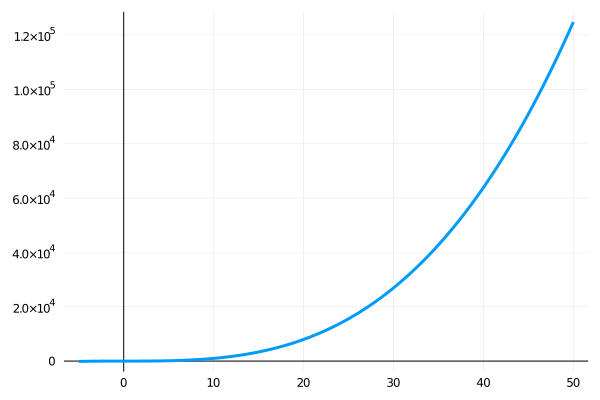
\includegraphics[width=10cm]{4}
        \caption{$f(x) = x^3 + 2.36995x^2 - 38.976263499999995x + 68.71088465$}
    \end{figure}

    \begin{center}
        Metoda Newtona
    \end{center}
    \begin{center}
        \begin{tabular}{|c|c|c|c|c|c|} 
            \hline
            Iteracja & $x_0$ & $f(x_0)$ & C.z. $x_0$ & C.z. $x_1$ & C.z. $x_2$ \\
            \hline
            1 & 2.0113803008969344 & 7.732777080647594 & 0 & 0 & 0 \\
            \hline
            5 & 0.4263474940328461 & 0.05932089727765367 & 1 & 1 & 1 \\
            \hline
            10 & 0.10692149626617695 & 7.912797366119274e-5 & 1 & 2 & 2 \\
            \hline
            15 & 0 & 0 & inf+ & inf+ & inf+ \\
            \hline
        \end{tabular}
    \end{center}
        
    \vspace{5mm}

    \begin{center}
        Metoda Bairstowa
    \end{center}
    \begin{center}
        \begin{tabular}{|c|c|c|c|c|c|} 
            \hline
            Iteracja & $x_0$ & $f(x_0)$ & C.z. $x_0$ & C.z. $x_1$ & C.z. $x_2$ \\
            \hline
            1 & 0.84033613 + 1.21947221im & -3.07751250 + 0.56499945im & 0 & inf+ & 0 \\ 
            \hline
            5 & 0.37452953 + 0.39006335im & 9.18010833055059e-5 & 1 & inf+ & 1 \\ 
            \hline
            15 & 0.10000018685790094 & 1.8685859924824825e-9 & 7 & inf+ & 3 \\
            \hline
            25 & 0.10000000000000013 & 1.2490009027033043e-18 & 15 & inf+ & 6 \\
            \hline
            40 & 0.1 & 0 & +inf & inf+ & 11 \\
            \hline
        \end{tabular}
    \end{center}

    \vspace{5mm}

    \begin{center}
        Błędy bezwzględne dla wzorów Cardano:
        \[
            e(x_0) = 0 \qquad e(x_1) = 2.3629366184170625e-10 \qquad e(x_2) = 2.3629364796391844e-10  
        \]
    \end{center}

\newpage
\subsection{Test 5}
Funkcja, o wybranych współczynnikach tak, aby oblczenia były 'niebezpieczne' numerycznie.
    \begin{figure}[h]
        \centering
        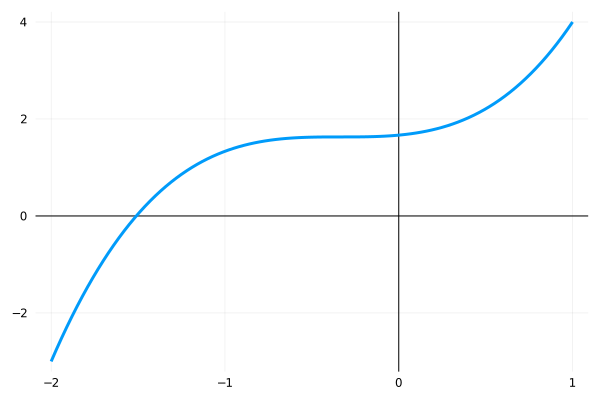
\includegraphics[width=10cm]{5}
        \caption{$f(x) = x^3 + 1.0000001038583122x^2 + 0.33333364701740337x + 1.6666667812898837$}
    \end{figure}

    \begin{center}
        Metoda Newtona
    \end{center}
    \begin{center}
        \begin{tabular}{|c|c|c|c|c|c|} 
            \hline
            Iteracja & $x_0$ & $f(x_0)$ & C.z. $x_0$ & C.z. $x_1$ & C.z. $x_2$ \\
            \hline
            1 & -1955.1001700352447 & -7.4693857239496355e9 & 0 & 0 & 0 \\
            \hline
            10 & -51.181437422003114 & -131467.652885827 & 0 & 0 & 0 \\
            \hline
            20 & -1.5770066485475038 & -0.29398900499360264 & 2 & 0 & 0 \\
            \hline
            25 & -1.510116082353336 & -2.97379159244366e-16 & 20 & 16 & 16 \\
            \hline
        \end{tabular}
    \end{center}
        
    \vspace{5mm}

    \begin{center}
        Metoda Bairstowa
    \end{center}
    \begin{center}
        \begin{tabular}{|c|c|c|c|c|c|} 
            \hline
            Iteracja & $x_0$ & $f(x_0)$ & C.z. $x_0$ & C.z. $x_1$ & C.z. $x_2$ \\
            \hline
            1 & -2.1962930904616655 & -4.835994078624513 & 0 & 0 & 0 \\ 
            \hline
            10 & -1.486247437 - 1.562610208im & 8.54254956 - 2.415611203im & 0 & 0 & 0 \\ 
            \hline
            20 & 0.5921042807 + 1.019336546im & -0.4625127 + 1.559847674im & 0 & 1 & 0 \\
            \hline
            25 & 0.2550579892 + 1.019123845im & 0 & inf+ & inf+ & inf+ \\
            \hline
        \end{tabular}
    \end{center}

    \vspace{5mm}

    \begin{center}
        Błędy bezwzględne dla wzorów Cardano:
        \[
            e(x_0) = 1.731027414741959e-7 \qquad e(x_1) = 6.924109678897218e-8 \qquad e(x_2) = 6.924109678897218e-8
        \]
    \end{center}    

\newpage
\subsection{Test 6}
Funkcja, dla której ciężko wybrać właściwe początkowe przybliżenie pierwiastka.
    \begin{figure}[h]
        \centering
        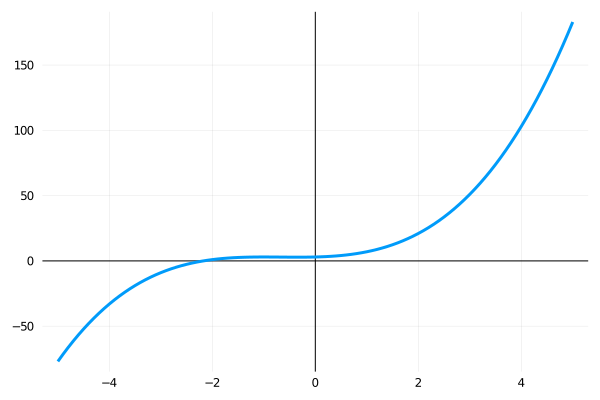
\includegraphics[width=10cm]{6}
        \caption{$f(x) = x^3 + 2x^2 + 1x + 3$}
    \end{figure}

    \begin{center}
        Metoda Newtona
    \end{center}
    \begin{center}
        \begin{tabular}{|c|c|c|c|c|c|} 
            \hline
            Iteracja & $x_0$ & $f(x_0)$ & C.z. $x_0$ & C.z. $x_1$ & C.z. $x_2$ \\
            \hline
            1 & 87.40256216597504 & 683055.1593426905 & 0 & 0 & 0 \\
            \hline
            5 & 16.732615031525334 & -131467.652885827 & 0 & 0 & 0 \\
            \hline
            10 & 1.5437877415713737 & 12.98962828477444 & 0 & 0 & 0 \\
            \hline
            20 & 4.263718879956009 & 121.1337352919147 & 0 & 0 & 0 \\
            \hline
            21 & 2.5950439877792135 & 36.53923411927553 & 0 & 0 & 0 \\
            \hline
            22 & 1.4381143629749316 & 11.548729387762949 & 0 & 0 & 0 \\
            \hline
            23 & 0.5468007419391421 & 4.308271373440125 & 0 & 0 & 0 \\
            \hline
            24 & -0.5080684029847669 & 2.8770491250635657 & 0 & 0 & 0 \\
            \hline
            25 & 10.648772161362636 & 1447.973348832624 & 0 & 0 & 0 \\
            \hline
            40 & 8.55818117413703 & 784.8653963832828 & 0 & 0 & 0 \\
            \hline
            48 & -2.182745085909218 & -0.05341140744611266 & 2 & 0 & 0 \\
            \hline
            49 & -2.1746057681803856 & -0.00030077451451259693 & 5 & 0 & 0 \\
            \hline
            50 & -2.174559411791341 & -9.721197942146932e-9 & 10 & 7 & 7 \\
            \hline

        \end{tabular}
    \end{center}
        
    \vspace{5mm}

    \begin{center}
        Metoda Bairstowa
    \end{center}
    \begin{center}
        \begin{tabular}{|c|c|c|c|c|c|} 
            \hline
            Iteracja & $x_0$ & $f(x_0)$ & C.z. $x_0$ & C.z. $x_1$ & C.z. $x_2$ \\
            \hline
            1 & 0.121495327 + 1.228746647im & -0.417133300 + 0.02512335599im & 0 & 0 & 0 \\ 
            \hline
            2 & 0.088623332 + 1.172063711im & -0.007673587 + 0.005065978im & 2 & 2 & 2 \\ 
            \hline
            3 & 0.087280433 + 1.171310438im & -0.4625127 + 1.559847674im & 5 & 4 & 5 \\
            \hline
            4 & 0.087279705 + 1.171312110im &  1.62191396e-11 + 2.4867478e-12im & 6 & 6 & 6 \\
            \hline
            5 & 0.087279705 + 1.171312111im &  1.36092529e-15 + 3.8459193e-16im & 15 & 13 & 13 \\
            \hline
            15 & 0.087279705 + 1.17131211im &  1.36092529e-15 + 3.8459193e-16im & 15 & 13 & 13 \\
            \hline
        \end{tabular}
    \end{center}

    \vspace{5mm}

    \begin{center}
        Błędy bezwzględne dla wzorów Cardano:
        \[
            e(x_0) = 1.3766765505351941e-14 \qquad e(x_1) = 9.90189642062563e-15 \qquad e(x_2) = 9.90189642062563e-15
        \]
    \end{center}
    
\newpage
\section{Wnioski i podsumowanie}
    \subsection{Metoda bisekcji}
        Metoda ta w żadnym teście nie uzyksała nawet 8 cyfr znaczących dla każdego pierwiastka, nawet
        pomimo tego, że ręcznie podałem jej dość mały początkowy przedział. Miało to zobrazować, dlaczego
        metoda ta nie jest zbyt użytecznym sposobem na wyliczanie pierwiastków wielomianu 3-go stopnia.
        Dodatkowo zera funkcji wolno zbiegają i średnio potrzebowały conajmniej 15 iteracji, aby uzyskać
        nawet słabe przybliżenia zer funkcji. Mimo to jest prosta w aplikacji i zrozumienia, więc może stanowić
        dobre tło dla innych metod.
        
    \subsection{Metoda Newtona}
        Metoda Newtona dużo lepiej radziła sobie ze znajdywaniem zer naszych funkcji w większości przypadków.
        W każdym teście metoda w najwyżej 20 iteracjach znajdywała bardzo dobre przybliżenia zer. Wyjątkiem był Test 6,
        w którym wyznaczone początkowe $x_0$ było bardzo nietrafione, co spowodowało, że metoda przez ponad 40 iteracji nawet
        nie zbliżała się do szukanej wartości. Jest to wynik bardzo niezadowalający nawet pomimo tego, że finalnie udało
        jej się to zero znaleźć. Musimy pamiętać jednak, że istnieją funkcje, dla których ta metoda nigdy nie będzie 
        zbiegać do miejsc zerowych funkcji, co oczywiście może mieć przykre konsekwencje przy rozwiązywaniu różnych problemów.
        
        Metoda ta więc może być przydatna tylko, jeśli znamy jakieś właności funkcji pozwalające określić punkt startowy,
        lub jeśli znamy same przybliżenia. W takim wypadku metoda jest jak najbardziej prawidłowa. Dla naszego problemu
        jednak, ten algorytm nie może być uznany jako numerycznie efektywny.
    \subsection{Wzory Cardano}
        Korzystanie ze wzorów Cardano jest oczywiście najszybszym sposobem na uzyskanie pierwiastków wielomianu, ponieważ
        polega na przeprowadzeniu konkretnej ilości, chociaż dość sporej, operacji arytmetycznych. Uzyskane wyniki są
        wyjątkowo dobrymi przybliżeniami naszych pierwiastków niemal w każdym przypadku i najczęściej błąd bezwzględny
        tych wartości jest zaniedbywalny. Istnieją jednak funkcje, których współczynniki mogą niestety dać przekłamane
        (choć nieznaczne) zera. Wtedy nasz błąd zwiększa się do rzędu $e-5$, a być może nawet więcej. Uważać więc trzeba,
        aby nasze wykonywane operacje nie obejmowały odejmowania dwóch bardzo bliskich liczb, gdyż może to prowadzić
        (zwłaszcza gdy używamy mniejszej precyzji bitowej) do błędnych wyników. Mimo tego, wzory Cardano są efektywnym
        sposobem na wyznaczanie pierwiastków wielomianów 3-go stopnia.
    \subsection{Metoda Bairstowa}
        Metoda Bairstowa była zdecydowanie najlepszą metodą do wyznaczanie pierwiastków wielomianów 3-go stopnia. Jest
        ona zbieżnie w każdym przypadku i nierzadko potrzeba niewielkiej ilośći iteracji, aby uzyskać bardzo satysfakcjonujące
        wyniki. Możemy oczywiście przeprowadzać dalsze iteracje, aby zwiększyć dokładność naszych zer, oczywiście z pewnym, ale sporym
        górnym ograniczeniem. Dodatkowo wybór dwóch startowych wartości, mimo że zmienia prędkość zbieżności, a czasem i błąd bezwzględny
        przybliżeń, nie jest problemem, gdyż bardzo łatwo je określić i dopasować do potrzeb zadania.

    \subsection{Podsumowanie}
        Z wybranch przeze mnie metod wyznaczania zer wielomianu 3-go stopnia najlepsza jest metoda Bairstowa, która
        ma wysoką zbieżność oraz wysoki poziom bezpieczeństwa przy uzysykiwaniu przybliżeń zer funkcji. 
        Być może udałoby się skonstruować bardziej konkretny sposób dla konkretynch zer funkcji, lecz byłoby to problematyczne
        w identyfikacji i implementacji. Dlatego to właśnie metodę Bairstowa zaproponowałbym jako sposób na 
        efektywne wyznaczanie zer funkcji takich wielomianów.
        
\begin{thebibliography}{9}
    \bibitem{Kincaid}
    David Kincaid, Ward Cheney. 
    Analiza numeryczna, Warszawa, 2006..
    \bibitem{Kincaid}
    Wikipedia:
    \texttt{https://pl.wikipedia.org/}
\end{thebibliography} 

\end{document}
